\documentclass{article}
\usepackage{amsmath}
\usepackage{amssymb}
\usepackage{graphicx}
\usepackage{hyperref}
\usepackage[version=4]{mhchem}


\begin{document}
\section*{Problem}
(AIME) Triangle \(A B C\) is isosceles, with \(A B=A C\) and altitude \(A M=\) 11. Suppose that there is a point \(D\) on \(A M\) with \(A D=10\) and \(\angle B D C=3 \angle B A C\). Then the perimeter of triangle \(A B C\) may be written in the form \(a+\sqrt{b}\), where \(a\) and \(b\) are integers. Find \(a+b\).\\
\centering
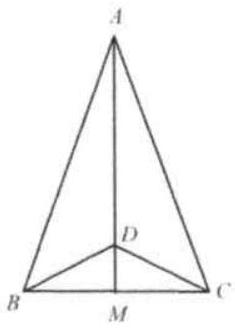
\includegraphics[width=\textwidth]{images/066.jpg}

\section*{Solution}
616.
Let the bisector of \(\angle A B D\) intersect \(A D\) at \(E\), and let \(x=\) \(B E=A E\). By the Pythagorean Theorem,

\[
B M=\sqrt{B E^{2}-E M^{2}}=\sqrt{x^{2}-(11-x)^{2}}=\sqrt{22 x^{2}-121}
\]

By applying the Pythagorean Theorem two more times, we find that \(A B=\sqrt{B M^{2}+A M^{2}}=\sqrt{22 x}\)

\[
B D=\sqrt{B M^{2}+D M^{2}}=\sqrt{22 x-120} .
\]

By the angle-bisector theorem, we have that \(\frac{A B}{B D}=\frac{A E}{D E}\)\\
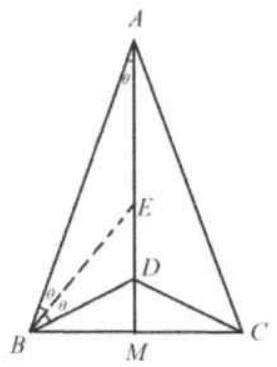
\includegraphics[width=\textwidth]{images/070(1).jpg} from which \(\frac{\sqrt{22 x}}{\sqrt{22 x-120}}=\frac{x}{10-x}\).\\
By squaring both sides of this equation and solving for \(x\), we find that \(x=55 / 8\). Hence \(B M=11 / 2\) and \(A B=(11 / 2) \sqrt{5}\). The perimeter of the triangle is \(2(A B+B M)=\)


\(11 \sqrt{5}+11=\sqrt{605}+11\), so \(a+b=616\).

\end{document}
